% chktex-file 44

\chapter{Methods}
\label{ch:methods}
This chapter presents the methodology of the proposed hybrid semantic exploration system, 
designed to mitigate the key limitations identified in Chapter~\ref{ch:sota}, namely the 
absence of persistent semantic memory, the reliance on single-source semantic detections, 
and the lack of an explicit and controllable trade-off between semantic exploration and 
exploitation in existing approaches.

The proposed system integrates zero-shot semantic perception with frontier-based exploration and persistent 3D semantic mapping into a unified, closed-loop decision-making framework. Semantic evidence acquired during exploration is continuously fused into a long-term spatial memory, while exploration behavior is adaptively modulated based on the reliability of accumulated semantic beliefs.

An overview of the system architecture is provided in Section~\ref{sec:methods:system_overview}, followed by detailed descriptions of the core components: semantic frontier exploration (Section~\ref{sec:methods:semantic_frontier}), promptable zero-shot detection (Section~\ref{sec:methods:zero_shot_detection}), persistent semantic 3D mapping (Section~\ref{sec:methods:persistent_mapping}), the multi-source fusion strategy governing semantic belief updates (Section~\ref{sec:methods:fusion_strategy}), and the behavior tree used to orchestrate semantic-guided exploration and navigation (Section~\ref{sec:methods:behavior_tree}).


\section{System Overview}
\label{sec:methods:system_overview}

The proposed system follows a modular hybrid architecture that tightly couples semantic perception,
geometry-driven exploration, and persistent semantic mapping to enable robust open-vocabulary
object-guided exploration. Figure~\ref{fig:system_overview} provides a high-level overview of the system components and their data flow. The exploration task is specified by a user-provided natural language prompt, which defines the semantic target and conditions the detection, exploration, and fusion modules throughout system execution.

\begin{figure}[h!]
    \centering
    \includegraphics[width=\textwidth]{Images/03_methods/sage_pipeline.png}
    \caption{Overview of the SAGE system architecture for open-vocabulary semantic exploration.
    RGB-D observations and robot poses are processed by three parallel modules: 
    (a) a persistent semantic mapping backend (OpenFusion~\cite{yamazakiOpenFusionRealtimeOpenVocabulary2023}) that maintains a semantic 3D map, 
    (b) a semantic frontier exploration module that scores geometric frontiers based on language-guided relevance, and 
    (c) a promptable zero-shot detection pipeline for object hypotheses.
    All semantic hypotheses are represented as graph nodes, filtered by relevance maps, and fused using a multi-source fusion strategy.
    A behavior tree orchestrates exploration, verification, and navigation actions, while low-level motion planning and execution are handled by the ROS~2 Navigation Stack~\cite{macenskiDesksROSMaintainers2023,makoviychukIsaacGymHigh2021}.}
\label{fig:system_overview}
\end{figure}

Robot observations at time $t$ are represented as RGB-D measurements $O_t = \{I_t, D_t\}$, where $I_t$ denotes the RGB image and $D_t$ the depth map. The robot pose in the world frame is denoted by $P_t$. To reduce computational load, observations are temporally and spatially downsampled prior to further processing.

The pre-processed observations are then fed into three parallel modules.
(a) The \textit{Memory Module} takes as input the current observations $O_t$ and pose $P_t$, obtained from the ROS~2 SLAM Toolbox~\cite{macenskiSLAMToolboxSLAM2021}, and updates the persistent semantic 3D map $M_t$.
(b) The \textit{Exploration Module} uses $O_t$ and $P_t$ to generate semantic frontiers $F_t$ from the current exploration occupancy grid.
(c) The \textit{Detection Module} processes $O_t$ to produce promptable zero-shot detections $D_t^{\text{det}}$.

Each module outputs a set of graph nodes representing semantic hypotheses.
Specifically, the memory module produces memory graph nodes $G_t^{\text{mem}}$ derived from the persistent map $M_t$, the exploration module outputs exploration graph nodes $G_t^{\text{exp}}$ corresponding to semantic frontiers $F_t$, and the detection module outputs detection graph nodes $G_t^{\text{det}}$ obtained from $D_t^{\text{det}}$.
This unified graph abstraction enables heterogeneous semantic hypotheses to be compared, filtered, and ranked using a common interface.

Prior to fusion, graph nodes are filtered using a relevance map to suppress nodes located in already explored areas. The remaining nodes are fused using the multi-source fusion strategy described in Section~\ref{sec:methods:fusion_strategy}, resulting in a unified set of weighted graph nodes $G_t^{\text{fused}}$.

Finally, the behavior tree described in Section~\ref{sec:methods:behavior_tree} selects the next high-level action based on $G_t^{\text{fused}}$, either navigating toward high-value frontiers for continued exploration or approaching detected objects for verification.
Low-level motion planning, obstacle avoidance, and execution are handled by the ROS~2 Navigation Stack~\cite{macenskiDesksROSMaintainers2023}.


\section{Semantic Frontier Exploration}
\label{sec:methods:semantic_frontier}

Semantic frontier exploration extends classical frontier-based exploration by incorporating
semantic relevance derived from vision-language models, enabling task-driven exploration guided by
a user-defined semantic prompt. Instead of exploring unknown space uniformly, the robot prioritizes frontiers that are more likely to yield observations relevant to the target concept~\cite{topiwalaFrontierBasedExploration2018, yamauchiFrontierbasedApproachAutonomous1997, yokoyamaVLFMVisionLanguageFrontier2023, alamaRayFrontsOpenSetSemantic2025}. Figure~\ref{fig:sage_maps} illustrates the intermediate map representations and processing stages used to construct the semantic frontier map.

\subsection*{Exploration Occupancy Maps}

The system maintains three distinct 2D occupancy grids for navigation and exploration:
(a) a SLAM map used for localization and navigation~\cite{macenskiSLAMToolboxSLAM2021},
(b) an exploration map used exclusively for frontier detection, and
(c) an inflated map that suppresses narrow passages and noisy frontier artifacts.
This separation decouples stable navigation from task-specific exploration decisions and prevents
semantic exploration logic from modifying the navigation map.

\begin{figure}[h!]
    \centering
    \includegraphics[width=\textwidth]{Images/03_methods/semantic_frontier_exploration/sage_maps.png}
    \caption{Overview of the map representations used for semantic frontier exploration.
    The SLAM map is used for localization and navigation, while the exploration map encodes
    task-specific explored and unexplored regions for frontier detection~\cite{macenskiSLAMToolboxSLAM2021}.
    An inflated map is used to suppress narrow structures and reduce spurious frontiers.
    The resulting frontier map is combined with a semantic value map to prioritize exploration
    toward semantically relevant regions.}
    \label{fig:sage_maps}
\end{figure}

Rather than running a separate SLAM instance for exploration, the exploration map is derived
directly from the SLAM occupancy grid~\cite{macenskiSLAMToolboxSLAM2021}.
Given the robot pose $P_t$ and the SLAM map $M_{\text{SLAM}}$, free space is raycast from the robot
into the occupancy grid, using the known sensor model and maximum sensor range, marking traversed cells as explored while preserving unknown regions beyond sensor reach. This raycasting process is applied to all recorded robot poses accumulated during the current task, yielding an exploration map $M_{\text{exp}}$ that reflects the explored workspace.

When a new semantic search task is initiated, all stored poses are cleared and the exploration map
is rebuilt from scratch, while the SLAM map remains unchanged.
This design ensures that exploration decisions are conditioned solely on task-relevant semantic
information and prevents bias from previously explored but semantically irrelevant regions.

\subsection*{Frontier Detection and Calculation}

Frontiers are defined as the boundary between known free space and unknown regions in the exploration occupancy grid~\cite{topiwalaFrontierBasedExploration2018} (see Figure~\ref{fig:frontier_detection}). This work uses the algorithm outlined in Algorithm~\ref{alg:extract_frontiers} to extract and cluster frontiers from the exploration map. 

\begin{figure}[h!]
    \centering
    \includegraphics[width=\textwidth]{Images/03_methods/frontier_example.png}
    \caption{Example of frontier detection on the exploration occupancy grid.
    Frontiers are identified as free cells adjacent to unknown space and clustered into spatially
    contiguous regions, with centroids serving as candidate exploration targets.}
    \label{fig:frontier_detection}
\end{figure}

Let $\mathcal{G} \in \{-1, 0, 100\}^{W \times H}$ denote the exploration occupancy grid, where $-1$ represents unknown space, $0$ free space, and $100$ occupied space~\cite{macenskiSLAMToolboxSLAM2021}. The set $\mathcal{F}_t$ denotes the set of detected frontier clusters at time step $t$. Each frontier cluster $\mathcal{P}$ is a set of spatially connected frontier cells. The set $\{\mathbf{c}_i^{t-1}\}$ contains the centroids of frontier clusters detected at the previous time step and is used to maintain temporal consistency via centroid matching.

\begin{algorithm}[H]
\caption{Geometric frontier extraction and clustering from the exploration occupancy grid}\label{alg:extract_frontiers}
\begin{algorithmic}[1]

\Function{ExtractFrontiers}{
    $\mathcal{G}$,
    $N_{\min}$,
    $N_{\max}$,
    $d_{\text{match}}$,
    $\{\mathbf{c}_{i}^{t-1}\}$
}
    \State $\mathcal{F}_t \gets \emptyset$ \Comment{Output set of clustered frontiers}

    \ForAll{cells $(x,y)$ with $\mathcal{G}(x,y)=0$} \Comment{Iterate over free cells}
        \If{$\mathcal{G}(x,y)=0$ \textbf{and} any 4-neighbor is unknown}
            \State Mark $(x,y)$ as frontier \Comment{Free–unknown boundary}
        \EndIf
    \EndFor

    \ForAll{unvisited frontier cells $(x,y)$}
        \State Grow a cluster $\mathcal{P}$ using 8-connected BFS
        \Comment{Spatially connected frontier region}

        \If{$N_{\min} \le |\mathcal{P}| \le N_{\max}$}
            \State Compute centroid $\mathbf{c} \gets \frac{1}{|\mathcal{P}|} \sum_{\mathbf{p} \in \mathcal{P}} \mathbf{p}$
            \Comment{Representative frontier location}

            \State Assign frontier ID via nearest centroid match within $d_{\text{match}} \in \mathbb{R}$

            \If{no match found}
                \State Assign new frontier ID \Comment{Newly discovered frontier}
            \EndIf

            \State Add $(\mathcal{P}, \mathbf{c})$ to $\mathcal{F}_t$
            \Comment{Store valid frontier}
        \EndIf
    \EndFor

    \State \Return $\mathcal{F}_t$ \Comment{Set of clustered, tracked frontiers}
\EndFunction

\end{algorithmic}
\end{algorithm}

The extracted frontier cells are clustered using an 8-connected \ac{BFS} to group spatially contiguous regions. Clusters that fall within predefined size limits ($N_{\min}$ and $N_{\max}$) are retained, while outliers are discarded.
Each valid frontier cluster is represented by its centroid, which serves as the candidate exploration target. Let $\mathcal{P} = \{\mathbf{p}_j \in \mathbb{R}^2 \mid j = 1,\dots,|\mathcal{P}|\}$ denote the set of grid cell coordinates belonging to a frontier cluster. The centroid $\mathbf{c} \in \mathbb{R}^2$ is defined as the arithmetic mean of the spatial coordinates of all cells belonging to the frontier cluster. Frontier identity matching is performed using nearest-neighbor association in Euclidean space, where a frontier centroid is assigned the ID of the closest previously observed centroid within distance $d_{\text{match}} \in \mathbb{R}$, otherwise a new frontier ID is created.

\begin{equation}
\label{eq:frontier_centroid}
\mathbf{c} = \frac{1}{|\mathcal{P}|} \sum_{\mathbf{p} \in \mathcal{P}} \mathbf{p}
\end{equation}

Equation~\ref{eq:frontier_centroid} yields a single representative location that approximates the geometric center of the frontier region. This centroid is used as the navigation target for frontier-based exploration and as the reference position for semantic
scoring.

The frontier centroids are tracked over time by matching them to previously detected frontiers based on spatial proximity, allowing for consistent identification of persistent frontiers across time steps. To extract the semantically most relevant frontiers, each frontier is scored using the value map generated by the \ac{VLM} as described below~\cite{yokoyamaVLFMVisionLanguageFrontier2023}. The scoring procedure is outlined in Algorithm~\ref{alg:value_map_query} and Algorithm~\ref{alg:semantic_frontier_update}. Let $\mathcal{C} = \{(x_i, y_i, s_i)\}$ denote the semantic value map represented as a set of 2D cells with associated semantic scores $s_i$, obtained by temporally aggregating cosine similarity values between vision-language model embeddings and the user-defined text prompt (Section~\ref{sec:semantic_frontier:value_map_generation}). For a value map cell $q \in \mathcal{C}$, $s(q)$ denotes the semantic similarity score stored at that cell.

\begin{algorithm}[H]
\caption{Value Map Mask for scoring Frontiers}
\label{alg:value_map_query}
\begin{algorithmic}[1]

\Function{GetScoreFromValueMap}{
    $\mathcal{C}$,
    $\mathbf{p}$
}
    \State $r \gets 0.3$ \Comment{Query radius}
    \State $s_{\max} \gets 0$
    \State $\text{observed} \gets \text{false}$
    
    \ForAll{points $q \in \mathcal{C}$}
        \If{$\lVert q - \mathbf{p} \rVert_2 < r$}
            \State $s_{\max} \gets \max(s_{\max}, s(q))$
            \Comment{Max semantic response}
            \State $\text{observed} \gets \text{true}$
        \EndIf
    \EndFor

    \If{$\text{observed}$}
        \State \Return $(\text{observed}=\text{true},\; \text{score}=s_{\max})$
    \Else
        \State \Return $(\text{observed}=\text{false})$
    \EndIf

\EndFunction

\end{algorithmic}
\end{algorithm}


The value map is a 2D grid in which each cell stores temporally aggregated cosine similarity scores
(see Section~\ref{sec:semantic_frontier:value_map_generation}) between \ac{VLM}
embeddings of scene observations and a user-defined text prompt.
Let $\mathcal{V} = \{(x_i, y_i, s_i)\}$ denote the value map, where $(x_i, y_i)$ are grid coordinates
and $s_i \in \mathbb{R}$ is the associated semantic similarity score.

To score a frontier, its centroid $\mathbf{c} \in \mathbb{R}^2$ is projected into the value map
coordinate frame.
The semantic score of the frontier is obtained by querying the maximum similarity score within a
fixed-radius neighborhood around $\mathbf{c}$, as described in
Algorithm~\ref{alg:value_map_query}.
If no valid score exists within this neighborhood, indicating that the region has not yet been
observed, the frontier is marked as unobserved.
Using the maximum response emphasizes strong semantic evidence while remaining robust to noise and
partial observations, consistent with prior semantic frontier scoring approaches~\cite{yokoyamaVLFMVisionLanguageFrontier2023}.

Algorithm~\ref{alg:semantic_frontier_update} summarizes the construction of semantic frontier graph
nodes by combining geometric frontier extraction with semantic scoring.

\begin{algorithm}[H]
\caption{Construction of semantic frontier graph nodes}
\label{alg:semantic_frontier_update}
\begin{algorithmic}[1]

\Function{UpdateSemanticFrontiers}{
    $\mathcal{G}$,
    $\mathcal{V}$,
    $\{\mathbf{c}_{i}^{t-1}\}$
}
    \State $\mathcal{F}_t \gets \textsc{ExtractFrontiers}(\mathcal{G}, N_{\min}, N_{\max}, d_{\text{match}}, \{\mathbf{c}_{i}^{t-1}\})$
    \Comment{Geometric frontier extraction}

    \ForAll{frontier $f \in \mathcal{F}_t$}
        \State $\mathbf{c} \gets \text{centroid}(f)$
        \Comment{Representative frontier position}

        \State $(\text{observed}, s) \gets \textsc{GetScoreFromValueMap}(\mathcal{V}, \mathbf{c})$
        \Comment{Semantic value lookup}

        \State Create graph node $n$
        \State $n.\text{id} \gets f.\text{id}$
        \State $n.\text{position} \gets \mathbf{c}$
        \State $n.\text{score} \gets s$
        \State $n.\text{observed} \gets \text{observed}$

        \State Add $n$ to graph
        \Comment{Semantic frontier node}
    \EndFor

    \State Publish frontier graph
    \Comment{For downstream task and visualization}

\EndFunction

\end{algorithmic}
\end{algorithm}

The final step involves creating graph nodes for each frontier, encapsulating their ID, position, semantic score, and observation status. These semantic frontier graph nodes form the primary input to the fusion strategy and behavior tree described in Sections~\ref{sec:methods:fusion_strategy} and~\ref{sec:methods:behavior_tree}.

\section*{Value Map Generation using Vision-Language Models}
\label{sec:semantic_frontier:value_map_generation}

The value map can be interpreted as an analogy to gradient ascent in deep reinforcement learning, where the robot seeks to maximize an expected semantic reward by navigating toward regions with high relevance to a target concept~\cite{yokoyamaVLFMVisionLanguageFrontier2023,gadreCoWsPastureBaselines2022,majumdarZSONZeroShotObjectGoal2023,thomasPolicyGradientMethods2017}. In this work, the value map represents the slope of a semantic reward function. In contrast to classical gradient ascent, movement toward regions of high semantic relevance is constrained by obstacles and unknown space. Consequently, geometrically derived frontiers serve as feasible navigation targets that guide the robot toward high-value regions while ensuring safe traversal, thereby preventing convergence to unreachable local maxima~\cite{gadreCoWsPastureBaselines2022}. Figure~\ref{fig:methods:gradient_ascent} illustrates this analogy, showing the semantic reward landscape and the role of frontier-based navigation (see Chapter~\ref{sec:methods:fusion_strategy} for the reward definition).

\begin{figure}[h!]
    \centering
    \includegraphics[width=\textwidth]{Images/03_methods/semantic_frontier_exploration/gardient_ascent.png}
    \caption{Conceptual visualization of the gradient-ascent analogy for semantic frontier exploration. Semantic relevance is illustrated as a folded reward surface, where frontier and memory graph nodes are elevated according to their semantic scores at position $(x,y)$.
    Geometric frontiers constrain feasible ascent directions under spatial obstacles.}
    \label{fig:methods:gradient_ascent}
\end{figure}

The value map is generated using a pre-trained vision-language model, specifically BLIP-2~\cite{liBLIP2BootstrappingLanguageImage2023}, which is queried via a ROS~2 service to compute semantic similarity between visual observations and a user-defined text prompt.
The value map node subscribes to RGB images, robot poses, and a global occupancy grid produced by a
LiDAR-based SLAM system. This differs from prior semantic frontier approaches such as VLFM~\cite{yokoyamaVLFMVisionLanguageFrontier2023}, which rely on depth camera projections and odometry-based local maps. By leveraging LiDAR-based SLAM, the proposed system maintains a globally consistent exploration map with reduced drift, enabling persistent semantic value accumulation over long trajectories. Figure~\ref{fig:methods:value_map_ros2_pipeline} illustrates the overall value map generation pipeline.

\begin{figure}[h!]
    \centering
    \includegraphics[width=\textwidth]{Images/03_methods/semantic_frontier_exploration/value_map_ros2_pipeline.png}
    \caption{ROS~2 value map generation pipeline using the BLIP-2 vision-language model for computing image-text cosine similarity.}
    \label{fig:methods:value_map_ros2_pipeline}
\end{figure}

Upon receiving an RGB image and a text prompt, the BLIP-2 service computes an image embedding and a text embedding using its pre-trained visual and textual encoders. The input image is divided into a grid of fixed-size patches, which are flattened, added with positional embeddings, and linearly projected before being processed by a vision transformer to capture spatial and semantic context~\cite{sharirImageWorth16x162021,liBLIP2BootstrappingLanguageImage2023}. Similarly, the text prompt is tokenized into subword units, embedded, and processed by a language transformer to model semantic and syntactic relationships.

Therefore, both embeddings are projected using learned projection matrices \( W_I \) and \( W_T \)
into a common embedding space (see Equation~\ref{eq:methods:value_map:projection}):

\begin{equation}
E_I = W_I f_I(I), \qquad
E_T = W_T f_T(T)
\label{eq:methods:value_map:projection}
\end{equation}

where \( f_I(\cdot) \) and \( f_T(\cdot) \) denote the visual and textual encoders, respectively.
The projection matrices \( W_I \) and \( W_T \) are learned during pre-training using an
\ac{ITC} objective, which optimizes the cosine similarity between matching
image-text pairs while pushing apart non-matching pairs~\cite{radfordLearningTransferableVisual2021,liBLIP2BootstrappingLanguageImage2023}. This training procedure aligns visual and textual representations in a shared semantic embedding space, enabling direct similarity comparison via cosine similarity. The projected embeddings are subsequently L2-normalized to unit length, which is required for cosine similarity computation.

The cosine similarity score \( S \) between the normalized image embedding \( \hat{E}_I \) and text embedding \( \hat{E}_T \) is computed as:

\begin{equation}
S = \hat{E}_I \cdot \hat{E}_T
  = \frac{E_I}{\|E_I\|_2} \cdot \frac{E_T}{\|E_T\|_2} = \cos(\hat{E}_I, \hat{E}_T)
\label{eq:methods:value_map:cosine_similarity}
\end{equation}

Figure~\ref{fig:methods:cosine_sim} illustrates this image-text similarity computation, where
visual observations are embedded by the BLIP-2 image encoder and compared against a
user-defined text prompt in a shared semantic embedding space. Although cosine similarity is theoretically bounded in the interval \([-1,1]\), in practice \ac{ITC}-based \acp{VLM} yield similarity scores concentrated in a narrow positive range~\cite{radfordLearningTransferableVisual2021,liBLIP2BootstrappingLanguageImage2023}. This continuous score serves as a measure of semantic relevance between the current visual observation and the target concept.

\begin{figure}[h!]
    \centering
    \includegraphics[width=\textwidth]{Images/03_methods/blip2_cosine_sim.png}
    \caption{Image-text cosine similarity computation using the BLIP-2 \ac{ITC} head.
    An RGB observation is embedded by the visual encoder and compared against a user-defined text prompt in a shared semantic embedding space~\cite{liBLIP2BootstrappingLanguageImage2023}.}
    \label{fig:methods:cosine_sim}
\end{figure}

\subsubsection*{Cosine Similarity to Value Map Projection}

The computed cosine similarity score is integrated into a persistent 2D semantic value map in a
pose- and visibility-aware manner.
Let $V_{t-1}$ denote the semantic value map and $C_{t-1}$ the associated confidence map at time
step $t-1$, and let $s_t$ be the cosine similarity score obtained from the \ac{VLM}
at the current robot pose $\mathbf{p}_t$.

The update procedure, summarized in Algorithm~\ref{alg:value_map_update}, consists of three
conceptual stages: (a) motion-gated temporal decay, (b) visibility-aware observation selection, and
(c) confidence-weighted fusion. The following update procedure closely follows the semantic value map formulation proposed in VLFM~\cite{yokoyamaVLFMVisionLanguageFrontier2023}, with adaptations for ROS~2 integration.

\begin{algorithm}[H]
\caption{2D Value Map Update using Vision-Language Model Similarity Scores}
\label{alg:value_map_update}
\begin{algorithmic}[1]

\Function{UpdateSemanticValueMap}{
    $V_{t-1}$,
    $C_{t-1}$,
    $s_t$,
    $\mathbf{p}_t$
}

    \State \algcomment{(a) Motion-gated temporal decay}
    \If{$\|\mathbf{p}_t - \mathbf{p}_{t-1}\|_2 > \delta_{\text{move}}$}
        \State $V_{t-1} \gets \lambda V_{t-1}$
        \State $C_{t-1} \gets \lambda C_{t-1}$
    \EndIf

    \State \algcomment{(b) Visibility and observation confidence}
    \State Compute visibility mask $M_{\text{fov}}(\mathbf{p}_t)$ via raytracing
    \State Compute confidence map $C_{\text{obs}}(\mathbf{p}_t, M_{\text{fov}})$

    \State \algcomment{(c) Confidence-weighted fusion}
    \ForAll{cells $(i,j)$ with $M_{\text{fov}}(i,j)=1$}

        \State $v \gets V_{t-1}(i,j)$
        \State $c \gets C_{t-1}(i,j)$
        \State $c_{\text{new}} \gets C_{\text{obs}}(i,j)$

        \If{$c + c_{\text{new}} = 0$}
            \State \textbf{continue}
        \EndIf

        \State $V_t(i,j) \gets v + \alpha\, c_{\text{new}} (s_t - v)$
        \State $C_t(i,j) \gets \max(\lambda c,\; c_{\text{new}})$

    \EndFor

    \State \Return $V_t,\; C_t$
\EndFunction
\end{algorithmic}
\end{algorithm}

(a) Temporal decay is applied to both the value map and the confidence map only if the robot
has translated more than a predefined threshold $\delta_{\text{move}}$ since the previous update.
This motion-gated decay prevents repeated observations from dominating the map when the robot
remains stationary or performs pure rotations, while still allowing outdated semantic evidence
to fade over time when the robot explores new regions. The decay factor
$\lambda \in [0,1]$ controls the persistence of past observations and prevents oscillation between multiple similar frontiers by gradually reducing the influence of stale semantic evidence when the robot revisits similar viewpoints~\cite{yokoyamaVLFMVisionLanguageFrontier2023}.

(b) The set of map cells that can be updated at time step $t$ is determined by computing a
top-down visibility mask $M_{\text{fov}}(\mathbf{p}_t)$ using raytracing within the current field
of view, instead of relying solely on depth camera projections based on odometry~\cite{yokoyamaVLFMVisionLanguageFrontier2023,thrunProbabilisticRobotics2006}. Only cells that are geometrically visible from the robot's pose and not occluded by obstacles are considered for update. For these visible cells, an instantaneous observation confidence map $C_{\text{obs}}(\mathbf{p}_t, M_{\text{fov}})$ is computed, which models the reliability of the current observation as a function of the sensor geometry. Cells near the center of the field of view are assigned higher confidence, while confidence decreases toward the periphery due to reduced resolution and increased distortion. This behavior is modeled using a Gaussian weighting function over the angular deviation from the camera’s principal viewing direction. The observation confidence assigned to a visible cell $(i,j)$ is computed as

\begin{equation}
\label{eq:value_map:confidence_weight}
C_{\text{obs}}(i,j)
=
\mathrm{e}^{-\frac{1}{2}
\left(
\frac{\Delta\theta(i,j)}{\sigma}
\right)^2},
\end{equation}

where $\Delta\theta(i,j)$ denotes the angular difference between the viewing ray toward cell
$(i,j)$ and the robot’s forward-facing direction, and $\sigma$ controls the sharpness of the
confidence decay within the field of view. Smaller values of $\sigma$ result in a narrower high-confidence region centered around the optical axis, while larger values produce a more uniform confidence distribution. This confidence formulation follows the angular weighting strategy used in VLFM to model observation reliability across the field of view~\cite{yokoyamaVLFMVisionLanguageFrontier2023}.


(c) For each visible cell $(i,j)$, the semantic value stored in the map is updated toward the
current similarity score $s_t$ using a confidence-weighted fusion rule.
Let $V_{t-1}(i,j)$ and $C_{t-1}(i,j)$ denote the semantic value and confidence stored at cell $(i,j)$
before the update, and let $C_{\text{obs}}(i,j)$ denote the instantaneous observation confidence
computed from the current field of view.

The semantic value update is formulated as a weighted interpolation between the previous value and
the current similarity score (see Equation~\eqref{eq:value_map:update}):

\begin{equation}
\label{eq:value_map:update}
V_t(i,j)
=
V_{t-1}(i,j)
+
\alpha\, C_{\text{obs}}(i,j)
\bigl(
s_t - V_{t-1}(i,j)
\bigr),
\end{equation}

where $\alpha \in [0,1]$ is an update gain that controls how strongly new observations influence the
existing value map. Higher observation confidence leads to a stronger correction toward the current similarity score, while low-confidence observations have only a minor effect. In parallel, the confidence map is updated to preserve strong observations over time. Specifically, the confidence assigned to each cell is defined in Equation~\eqref{eq:value_map:confidence_update}:

\begin{equation}
\label{eq:value_map:confidence_update}
C_t(i,j)
=
\max\!\bigl(
\lambda\, C_{t-1}(i,j),
\;
C_{\text{obs}}(i,j)
\bigr),
\end{equation}

where $\lambda \in [0,1]$ is the temporal decay factor applied when the robot has translated since
the previous update. Using a max operation ensures that regions which have been observed with high confidence remain influential even after decay, preventing repeated low-confidence observations from diluting reliable semantic evidence~\cite{yokoyamaVLFMVisionLanguageFrontier2023}.

Together, Equations~\eqref{eq:value_map:update} and~\eqref{eq:value_map:confidence_update} implement
a persistent, confidence-aware fusion mechanism that incrementally integrates semantic similarity
scores into a spatially consistent value map.

Figure~\ref{fig:methods:value_map:example} illustrates a generated value map for the prompts ``Bed'', ``TV'', and the zero-shot prompt ``A door leading to a bed'', demonstrating how prompt design can bias exploration toward multiple targets or semantically useful transition regions.


\begin{figure}[h!]
    \centering
    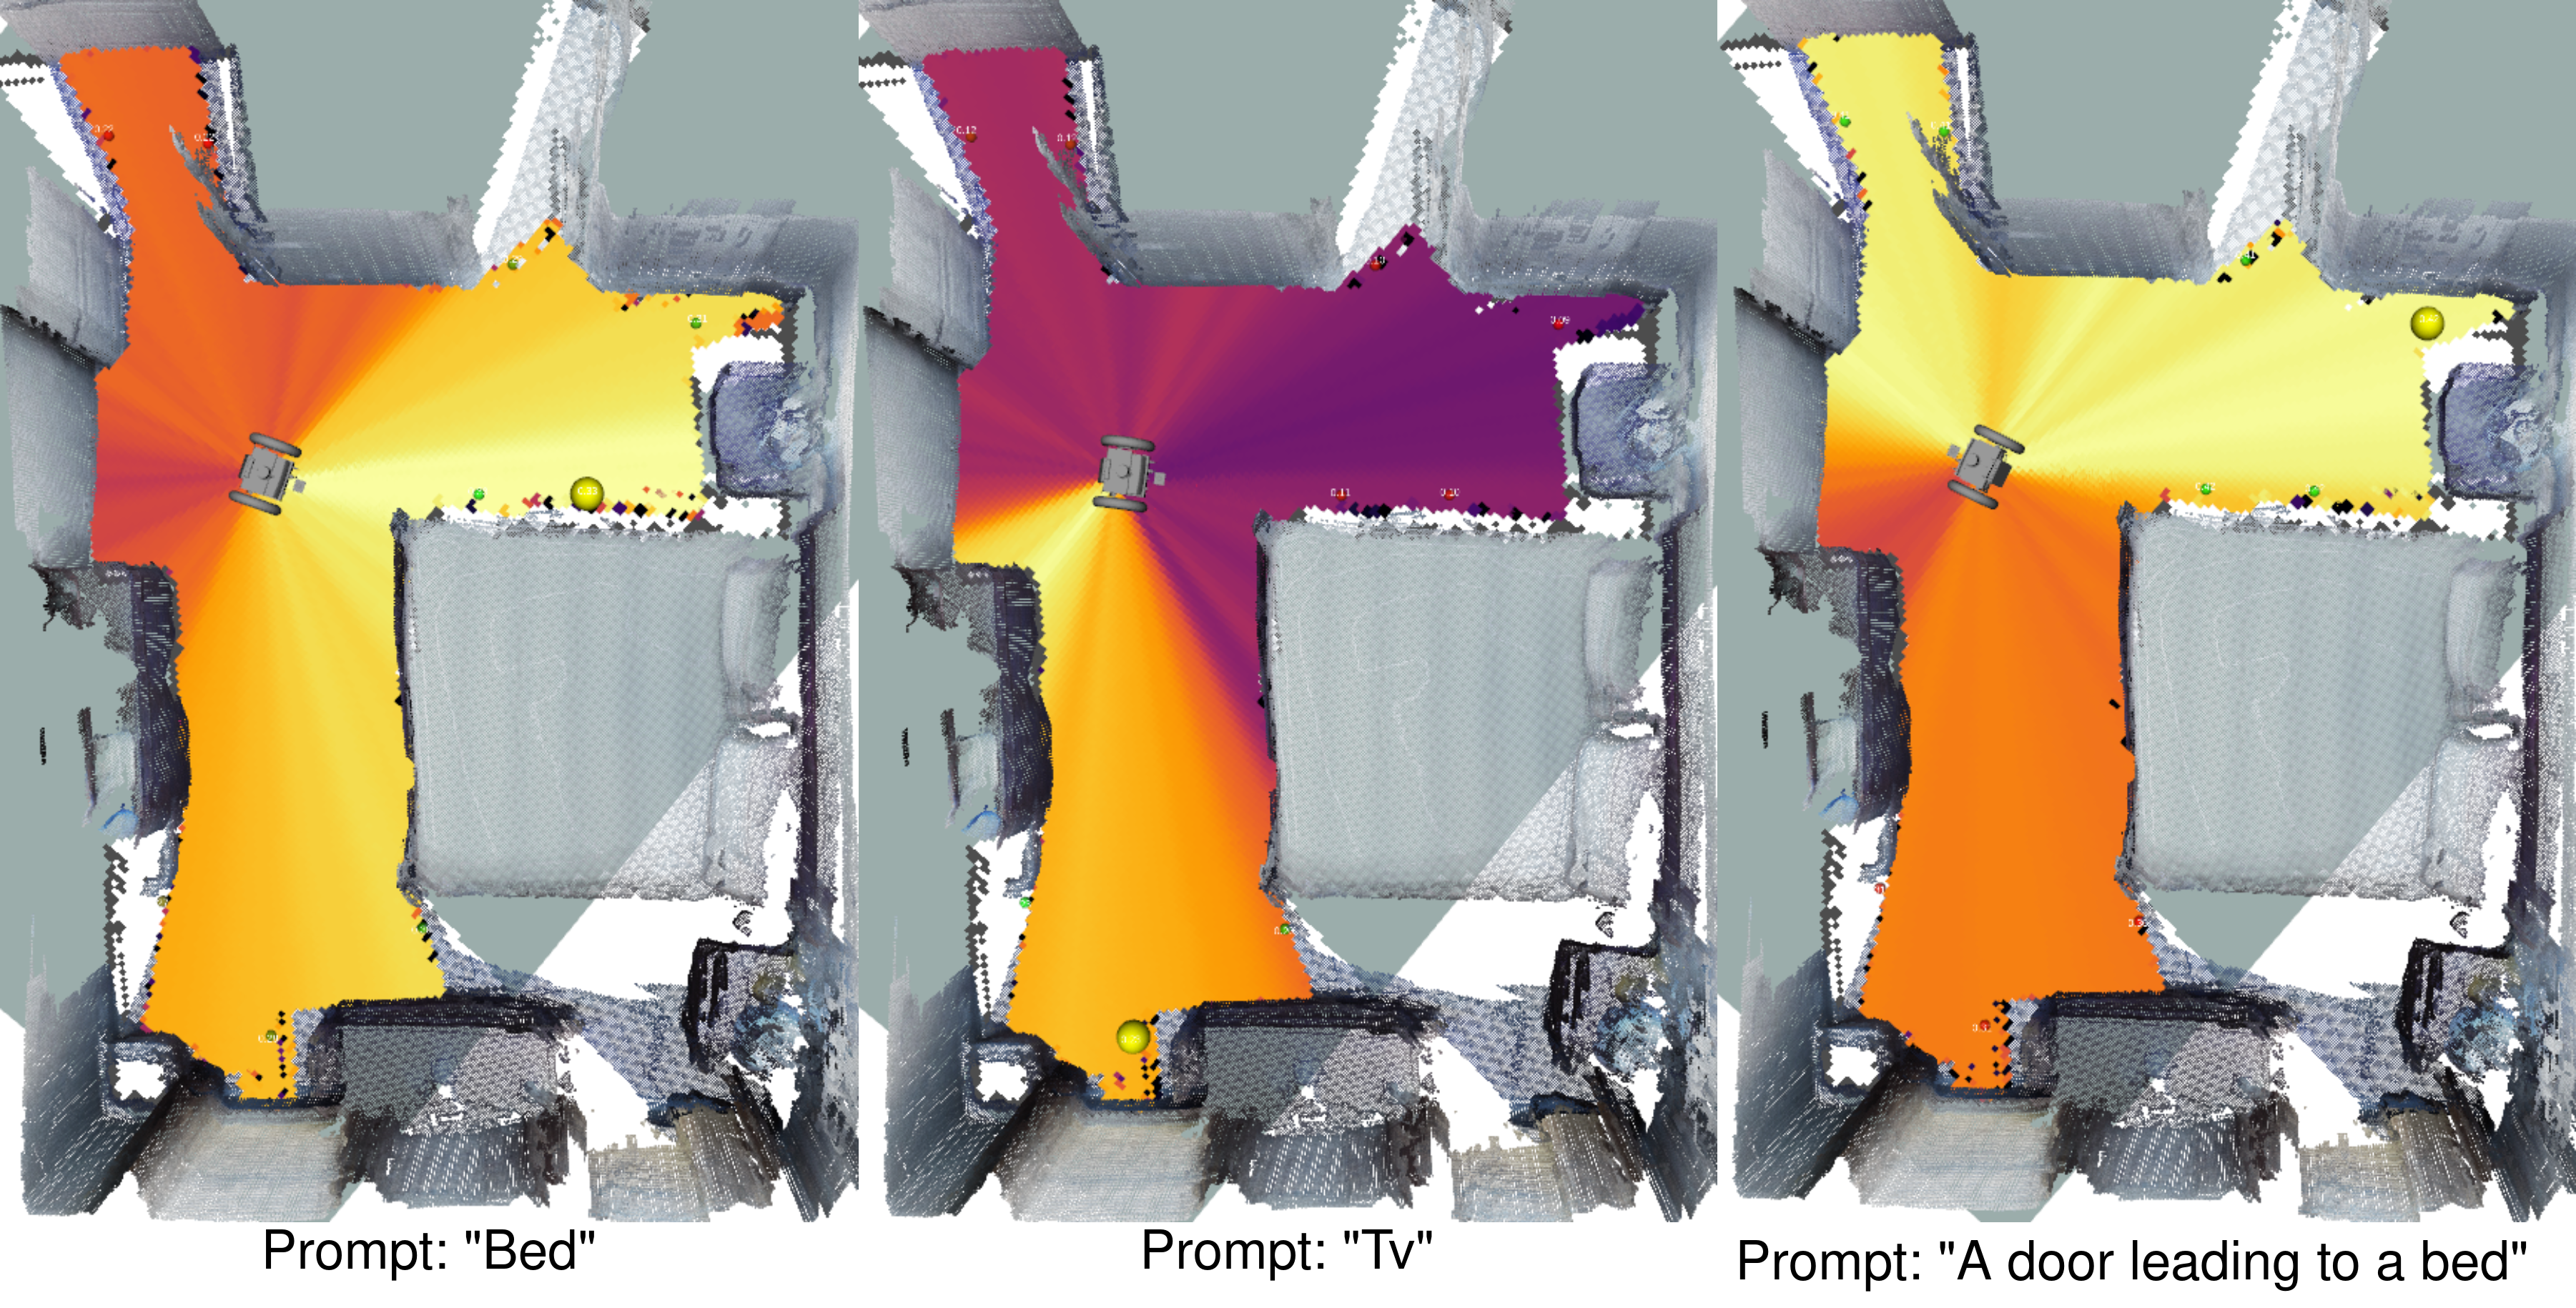
\includegraphics[width=\textwidth]{Images/03_methods/value_map_example.png}
    \caption{Example value maps generated using BLIP-2 for different text prompts.
    The value maps highlight regions of high semantic relevance to the prompts ``Bed'', ``TV'', and ``A door leading to a bed''.}
    \label{fig:methods:value_map:example}
\end{figure}

These scored frontiers are then encapsulated as graph nodes and passed to the fusion strategy
(Section~\ref{sec:methods:fusion_strategy}) for integration with memory and detection modules.

\section{Persistent Semantic 3D Mapping} 
\label{sec:methods:persistent_mapping}

The frontier centroids serve as a local guidance, which area should be explored next. However, to effectively search for multiple objects over extended periods, the robot requires a persistent memory of previously detected objects and their locations. This is achieved through a semantic 3D mapping module that constructs a global semantic point cloud map from RGB-D observations and generates object-level hypotheses as graph nodes. These memory graph nodes are then integrated into the fusion strategy (Section~\ref{sec:methods:fusion_strategy}) to inform exploration and detection decisions.

At the time implementation, OpenFusion~\cite{yamazakiOpenFusionRealtimeOpenVocabulary2023} was the most promising open-source framework for real-time semantic 3D mapping. Its trade-off between mapping accuracy, semantic integration, and computational efficiency made it suitable for onboard deployment on mobile robots with limited processing power. From the analysis of the state-of-the-art (see Chapter~\ref{sec:sota:semantic_scene_reconstruction}), shows zero-shot and realtime capabilities. However, OpenFusion is not object centric. Therefore, this work extends OpenFusion with object-level semantic clustering and graph node generation to create a persistent memory suitable for multi-object search tasks.

\subsection*{Global Map Construction with Open-Fusion}

OpenFusion~\cite{yamazakiOpenFusionRealtimeOpenVocabulary2023} originally focueses on offline semantic mapping using pre-recorded RGB-D sequences from for example the ScanNet dataset~\cite{daiScanNetRichlyannotated3D2017} or Replica dataset~\cite{straubReplicaDatasetDigital2019}. This work adapts OpenFusion for online operation on a mobile robot by integrating it with a LiDAR-based SLAM system for accurate global pose estimation. The OpenFusion ROS~2 wrapper subscribes to RGB-D images, camera intrinsics and robot poses, which are filtered (see Figure~\ref{fig:methods:persistent_mapping:pipeline}). Let the input pairs defined as $\{(I_t, D_t, P_t) \mid t = 1,\dots,K\}$, where $I_t$ is the RGB image, $D_t$ is the depth image, and $P_t$ is the robot pose at time step $t$. OpenFusion has a maximum number of voxel blocks that can be stored in memory. Therefore, the pose-rgbd pair is only passed to OpenFusion if the robot has moved more than a predefined threshold $\delta_{\text{move}}$ since the last update and is significantly different to all previous stored poses to avoid redundant observations. OpenFusion initializes with the current camera intrinsics, voxel size and voxel count, which represent entire available memory for the semantic map. For each accepted input pair, OpenFusion integrates the RGB-D observation into a global Truncated Signed Distance Function (TSDF) volume using the provided robot pose for accurate alignment. The wrapper openfusion_ros publishes continously the constructed pointcloud and on each prompt, it triggers the semantic mapping process. The semantic mapping calculates the with the users text prompt the text embedding and compares it to the visual embeddings and the top-k similar embeddings are used to label the points in the pointcloud with semantic labels and confidence scores. This enables a zero-shot semantic mapping capability, allowing the robot to build a semantic map tailored to arbitrary user-defined concepts without requiring prior training on specific object categories.

\begin{figure}[h!]
    \centering
    \includegraphics[width=\textwidth]{Images/03_methods/semantic_mapping/openfusion_ros_pipeline.png}
    \caption{}
    \label{fig:methods:persistent_mapping:pipeline}
\end{figure}

openfusion_ros outputs four poitclouds, first the 3D reconstruction pointcloud without semantic labels, second the pointcloud clusters which allign with the query prompt, third a semantic pointcloud, which requieres a list of classes to segment the pointcloud and fourth a panoptic pointcloud, which segments the pointcloud into different object instances. The difference between semantic and panoptic pointcloud is, that the semantic pointcloud only segments the pointcloud into different classes, e.g. chair, table, bed, while the panoptic pointcloud segments the pointcloud into different object instances, e.g. chair 1, chair 2, table 1. The semantic pointcloud and panoptic pointcloud are obtained with a ROS~2 service call, where the path of the classes json file is passed as argument. The classes json file contains a list of classes, which are used to segment the pointcloud. For example, if the user wants to search for chairs and tables, the classes json file contains the classes "chair" and "table". With the service call, the user can save the semantic and panoptic pointclouds on demand (further Information in Chapter~\ref{sec:implementation:evaluation}).

Now this returns a semantic pointcloud with semantic labels and confidence scores for each point. However, to create object-level hypotheses suitable for multi-object search tasks, the pointcloud is further processed to cluster points spatially.


\subsection*{Semantic Clustering and Graph Node Generation}
% \begin{itemize}
%     \item Clustering of points with similar semantic labels to form object-level hypotheses.
%     \item Construction of semantic graph nodes representing detected object instances with aggregated confidence scores.
%     \item Maintenance of the semantic graph as a persistent memory for multi-object search tasks.
% \end{itemize}

\section{Promptable Zero-Shot Detection} 
\label{sec:methods:zero_shot_detection}
\begin{itemize}
    \item In this work YOLO-E \cite{wangYOLOERealTimeSeeing2025} is used as the promptable zero-shot detection model.
    \item YOLO-E has the following advantages:
    \begin{itemize}
        \item High inference speed suitable for real-time applications.
        \item Ability to handle open-vocabulary object detection based on text prompts.
        \item Integration of both visual and textual information for robust detection.
        \item Pre-trained on large-scale datasets, enabling zero-shot generalization to unseen object categories.
    \end{itemize}
\end{itemize}


\subsection*{Open-Vocabulary Object Detection with YOLO-E}
\begin{itemize}
    \item Utilization of the YOLO-E model for open-vocabulary object detection based on text prompts.
    \item Extraction of 2D bounding boxes and associated confidence scores for detected objects.
    \item Segmentation of detected objects to isolate relevant pixels for 3D localization.
\end{itemize}

\subsection*{Depth-Based 3D Localization}
\begin{itemize}
    \item With camera intrinsics and depth information, the 2D bounding boxes ans segmentation masks are projected into 3D space.
    \item Calculation of 3D coordinates for each detected object using depth values within the bounding box.
    \item Semantic detection pointclouds are passed are then clustered and the centroid of each cluster is computed to obtain robust 3D object locations.
    \item For each cluster, the mean of the confidence scores of the associated 2D detections is calculated to assign a confidence score to the 3D localization.
\end{itemize}

\begin{figure}[h!]
    \centering
    \includegraphics[width=1.0\textwidth]{Images/03_methods/vlm_detector.png}
    \caption{YOLO-E detection to graph node 3D localization}
    \label{fig:vlm_detector}
\end{figure}


\section{Fusion Strategy}
\label{sec:methods:fusion_strategy}
\subsection*{Exploration–Memory Weighting}
\begin{itemize}
    \item Exploration and memory graph nodes are fused and weighted as follows:
    \begin{itemize}
        \item Proximity weighting: Nodes closer to the robot's current position are given higher weights, similar to~\cite{bourgaultInformationBasedAdaptive2002}.
        \item Exploration vs Memory: Nodes from the exploration source are prioritized over memory nodes to encourage discovery of new information, similar to~\cite{ramakrishnanPONIPotentialFunctions2022}.
        \item Costmap weighting: Nodes located in areas with lower navigation costs are favored to optimize path planning and navigation efficiency, similar to~\cite{bourgaultInformationBasedAdaptive2002}.
    \end{itemize}
\end{itemize}

\subsection*{Multi-Source Detection Fusion}
\begin{itemize}
    \item Detection graph nodes are weighted based on:
    \begin{itemize}
        \item YOLO-E confidence scores: Higher confidence detections are given more weight.
        \item BLIP-2 value map: Detections with higher semantic relevance to the text prompt are prioritized.
        \item The nearer detection graph nodes are to memory graph nodes, the higher their weight.
    \end{itemize}
\end{itemize}

\subsection*{Relevance Filtering and Node Suppression}
\begin{itemize}
    \item Each source's graph nodes are filtered based on a relevance threshold to eliminate graph nodes within the fov map.
    \item Relevance map is build over time
    \item If a graph node is located in an area that has already been explored and found to be irrelevant to the prompt, it is suppressed.
\end{itemize}

\begin{figure}
    \centering
    \includegraphics[width=1.0\textwidth]{Images/03_methods/3d_relevance_map.png}
    \caption{Fusion strategy for exploration, detection, and memory graph nodes}
    \label{fig:3d_relevance_map}
\end{figure}

\begin{figure}
    \centering
    \includegraphics[width=1.0\textwidth]{Images/03_methods/relevance_map_example.png}
    \caption{Fusion strategy for exploration, detection, and memory graph nodes}
    \label{fig:relevance_map_example}
\end{figure}

\section{Behavior Tree for Semantic-Guided Exploration} 
\label{sec:methods:behavior_tree}

\subsection*{High-Level Task Structure}
\begin{itemize}
    \item The behavior tree (BT) is designed to manage the high-level task structure for semantic-guided exploration.
    \item The BT consists of the following main components:
    \begin{itemize}
        \item Initialization: Clearing Maps, Publishing Prompts
        \item Detection Branch: If object is detected over a threshold, navigate to it, realign to object take picture
        \item Exploration Branch: While object not detected, perform semantic frontier exploration navigating to highest valued frontiers or memory nodes
        \item Termination: If object found, end mission; If time limit reached, end mission
        \item Behavior tree is called with a ros2 action server, which returns on termination success or failure, and actual path taken
    \end{itemize}
\end{itemize}

\begin{figure}[h!]
    \centering
    \includegraphics[width=0.5\textwidth]{Images/03_methods/sage_bt_flowchart.png}
    \caption{System architecture}
    \label{fig:system_overview}
\end{figure}

\subsection*{Integration with Navigation Stack}
\begin{itemize}
    \item Navigation stack used for low-level path planning and obstacle avoidance.
    \item Action used: navigate\_to\_pose, Spin
\end{itemize}
    
\newpage